\documentclass[12pt,a4paper]{article}
\usepackage{algorithm, algpseudocode, amsmath, amssymb, amsthm, bm, csquotes, emf, empheq, geometry, graphicx, hyperref, listings, mhchem, multirow, siunitx, caption, float, longtable}
\usepackage[italicdiff]{physics}
\usepackage[section]{placeins}
\usepackage[justification=centering]{caption}
\usepackage[column=O]{cellspace}
% \usepackage[extrafootnotefeatures]{xepersian}
\hypersetup{colorlinks=true, urlcolor=cyan}

\title{Solving Diffrential Equations with different methods\\
Capacitor Equation and Simple Harmonic Ocillator}

\author{Zahra Akbari}
\date{}


% \settextfont{}
\linespread{1.2}

\setlength\cellspacetoplimit{5pt}
\setlength\cellspacebottomlimit{3pt}
\newcommand{\multlinecell}[1]{\begin{tabular}[c]{@{}c@{}}#1\end{tabular}}

\newcommand{\qfrac}[2]{\left(\frac{#1}{#2}\right)}
\newcommand{\fsqrt}[2]{\sqrt{\frac{#1}{#2}}}
\newcommand{\ddfrac}[2]{{\displaystyle\frac{\displaystyle #1}{\displaystyle #2}}}
\newcommand{\pdvc}[3]{\qfrac{\partial #1}{\partial #2}_{#3}}
\newcommand{\dbar}{{d\mkern-7mu\mathchar'26\mkern-2mu}}
\newcommand*{\defeq}{\mathrel{\vcenter{\baselineskip0.5ex \lineskiplimit0pt
			\hbox{\scriptsize.}\hbox{\scriptsize.}}}
	=}

\begin{document}
	\maketitle
	\section{Solving RC Circuit Diffrential Equation }
	\subsection*{Analytical Solution}
	In a circuit with a capacitor, we got the following formula:
	\begin{align*}
		V_0-\frac{q}{c} &= IR \\
		\frac{dq}{dt} &= \frac{V_0}{R} - \frac{q}{RC}
	\end{align*}
	we define
	\begin{align*}
		q_0 &= Cv
	\end{align*}
	therefore:
	\begin{align*}
		q(t)&=q_0 (1-e^{-\frac{t}{RC}})
	\end{align*}
% \pagebreak

	\subsection*{Numerical Methods}
	For solving the diffrential equation we use the Euler Method and another idea resulting in unstable results.
	In this method we use the following relation:
	\begin{align*}
		y_{n+1} &= y_n (time step) F(x_n)
	\end{align*}
	where F is the derivite of y with respect to time. Initial values are considered for charging a capacitor. Therefore $q_0=0$ and R and C are also considered to be 1. The results for time step= 0.1 is shown below.

			
			\begin{figure}[H]
				\centering
				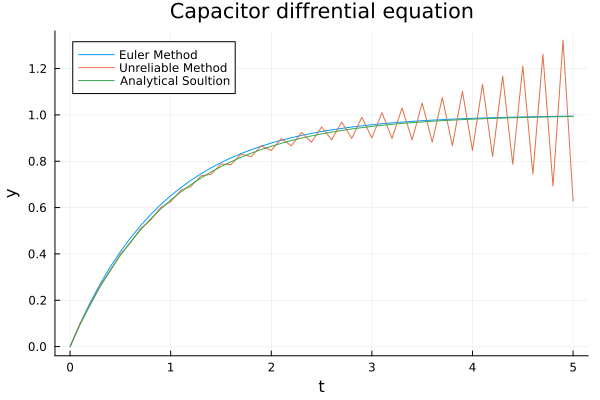
\includegraphics[width=10cm]{unstable.png}
				\caption{Comparing Euler and the unstable method. }
			\end{figure}
	The error of the Euler Method is also calculated using the mean least squares. The error increases with larger time steps:
	\begin{figure}[H]
		\centering
		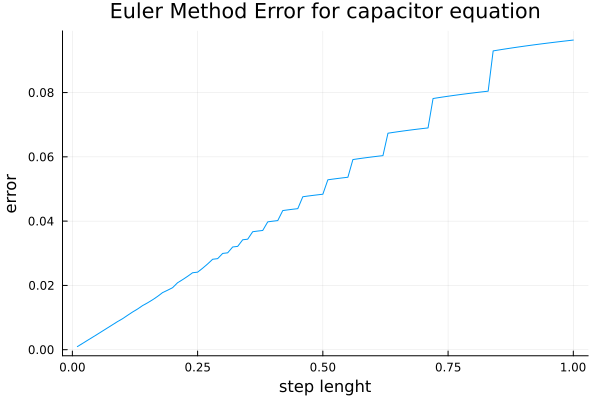
\includegraphics[width=10cm]{error.png}
		\caption{Euler Method error}
	\end{figure}

			

	\section{Simple Hrmonic Ocillator}		
			For the simple harmonic Ocillator we have:
			\begin{equation*}
				\ddot{x} = -\omega x 
			\end{equation*}
			Assuming the initial state to be starting from $dot{x}(0)=0$ : 
			\begin{align*}
				\dot{x} &= x_0 sin(\omega t) \\
				x &=  x_0 cos(\omega t)
			\end{align*}
			\subsection*{Solutions}
			For solving this diffrential equation The Euler, Euler-Cromers, LeapFrog, Verlet, Velovity Verlt and Beeman is used with 0.1 times step.
			The results are as follows:
			\begin{figure}[H]
				\centering
				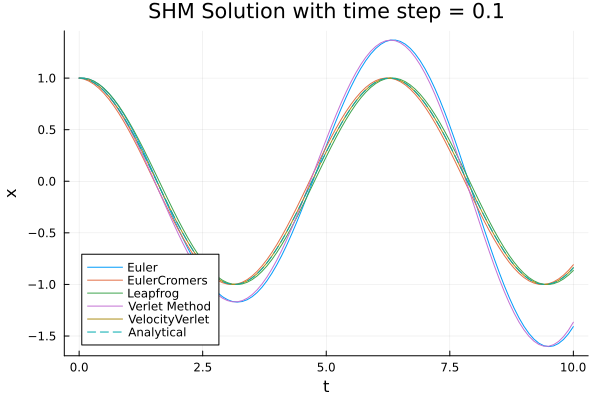
\includegraphics[width=10cm]{all.png}
				\caption{Simple Harmonic ocillator solved with different methods }
			\end{figure}

			\begin{figure}[H]
				\centering
				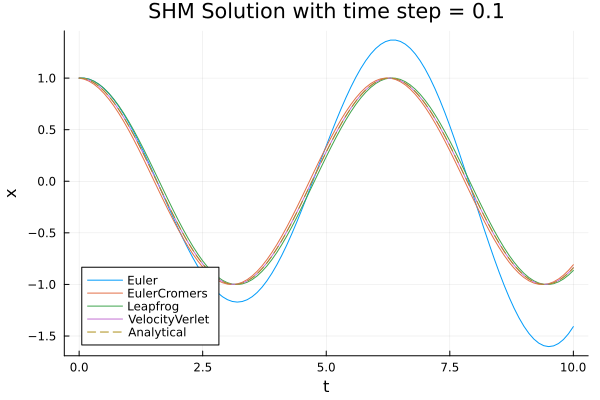
\includegraphics[width=10cm]{graph.png}
				\caption{Simple Harmonic ocillator solved with different methods }
			\end{figure}
			\begin{figure}[H]
				\centering
				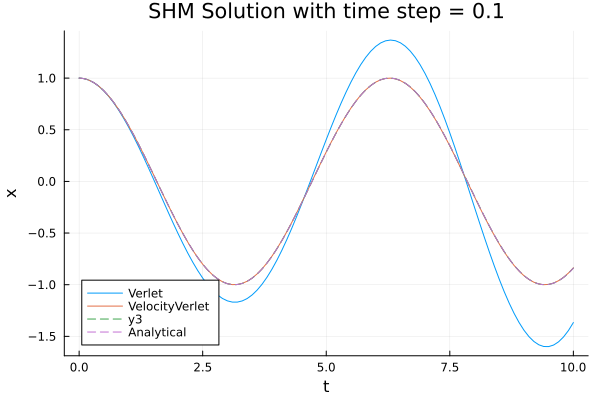
\includegraphics[width=10cm]{verlet.png}
				\caption{Comparing verlet and velocity verlet }
			\end{figure}
			\pagebreak
			
			\subsection*{Phase Space}
			Velocity Verlet seems to be the most accurate method, While Leapfrog and Euler-Cromers look almost similar in terms of accuracy. Beeman seems to be the least accurate. 
			\\
			The verlet method is unstable in this case, while Velocity Verlet is the best in terms of energy conservation.
			\begin{figure}[H]
				\centering
				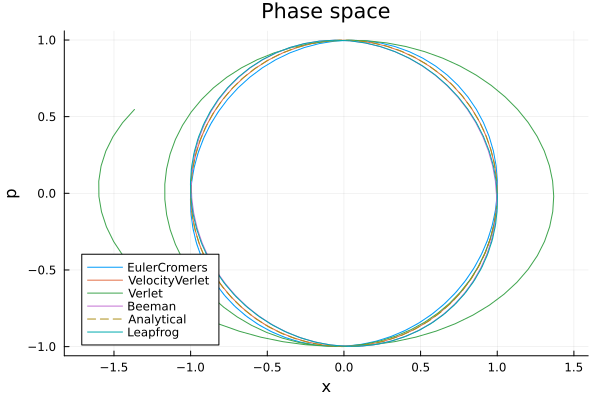
\includegraphics[width=10cm]{phase.png}
				\caption{Phase space and different methods }
			\end{figure}
			\end{document}
